\documentclass{beamer}
% begin handouts 
%\documentclass[handout]{beamer}
%\usepackage{pgfpages}
%\pgfpagelayout{4 on 1}[a4paper,border shrink=5mm,landscape]
% end   handouts

\usepackage{beamerthemesplit}
\usepackage{verbatim}
\usepackage{url}
 
%\usetheme{Bergen}
%\usetheme{Berlin} % se ven bien los nombres de autores
%\usetheme{Darmstadt}
\usetheme{Dresden} % se ven bien los nombres de autores
%\usetheme{Goettingen} %cosas raras, pero interesante igual
%\usetheme{Marburg} %cosas raras, pero interesante igual 
%\usetheme{Szeged}

\title{Buti\'a: Plataforma rob\'otica gen\'erica para la ense\~nanza de la inform\'atica}
\author[\Tiny{G. Tejera \and A. Aguirre \and F. Andrade \and P. Gindel \and S. Margni \and G. Reisch \and J. Visca}]{Gonzalo Tejera \and Andr\'es Aguirre \and \\~\\ Federico Andrade \and Pablo Gindel \and Santiago Margni \and Guillermo Reisch \and Jorge Visca}
\institute[InCo]{
\tiny{Instituto de Computaci\'on, Facultad de Ingenier\'ia, Universidad de la Rep\'ublica\\J. Herrera y Reissig 565, Montevideo, Uruguay\\
\href{http://www.fing.edu.uy/inco/proyectos/butia}{http://www.fing.edu.uy/inco/proyectos/butia} \\
\texttt{butia@fing.edu.uy}
}}

\date{28/03/2011}

\begin{document}

\frame{\titlepage}

\pgfdeclareimage[height=0.5cm]{congres-logo}{graphics/campus_logo.png}
\pgfdeclareimage[height=0.5cm]{butia-logo}{graphics/butia_logo.jpg}

\logo{\pgfuseimage{congres-logo}}

\setbeamertemplate{sidebar left}
{
\logo{\pgfuseimage{butia-logo}}
\vfill%
\rlap{\hskip0.1cm\insertlogo}%
\vskip9pt%
}
	
%\setbeamertemplate{navigation symbols}{} 
\setbeamertemplate{table of contents}{}

\section[Agenda]{}
\frame{\tableofcontents}


\setbeamertemplate{background canvas}{}

\section{Introducci\'on}
\subsection{Objetivos}
%FA
\begin{frame}
  \frametitle{Proyecto Buti\'a}
  \begin{center}
    \begin{itemize}
	    \item Crear una plataforma simple y econ\'omica que permita a alumnos de liceos p\'ublicos interiorizarse con la programaci\'on del comportamiento de robots
	    \item<2-> A trav\'es de la rob\'otica transmitir a profesores y estudiantes conocimientos b\'asicos sobre las nuevas tecnolog\'ias y sus aplicaciones
		\item<3-> Romper asimetr\'ia entre liceos p\'ublicos y privados
		\item<4-> El proyecto fue financiado por la ANII y apoyado por la unidad de extensi\'on de la Facultad de Ingenier\'ia
	\end{itemize}
    \end{center}
\end{frame}


 \frame {
  \frametitle{Rob\'otica Educativa}
  \begin{center}
	\begin{itemize}
	    \item Programar los comportamientos de un robot m\'ovil genera mucho inter\'es en los adolescentes
	    \item<2-> Permite alcanzar resultados visuales inmediatos de sus programas
        \item<3-> Se estimula la creatividad
		\item<4-> Aprendizaje de conceptos b\'asicos de programaci\'on
	\end{itemize}
  \end{center}
}

\frame {
  \frametitle{Proyecto OLPC (One Laptop per Child)}
  \begin{center}
%	   \begin{right}
		   \begin{figure}
			 	 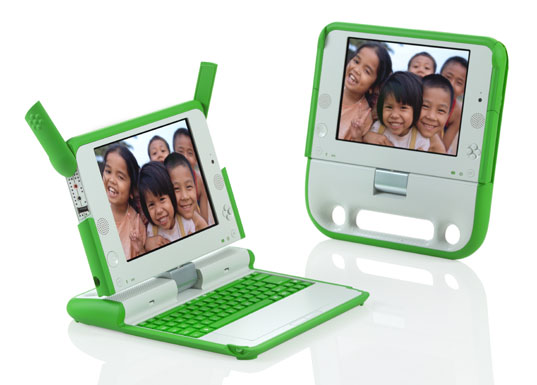
\includegraphics[scale=0.15]{graphics/xos.jpg}
		   \end{figure}
%	   \end{right}
	\begin{itemize}
	    \item El proyecto OLPC busca llevar una computadora con conectividad a cada ni\~no
	    \item<2-> Software: GNU/Linux y Sugar
        \item<3-> Hardware: Netbook de bajo consumo (computadora XO)
		\item<4-> En Uruguay es llevado a cabo por el plan Ceibal en primaria y secundaria
	\end{itemize}
  \end{center}
}

\frame {
  \frametitle{Transformando la XO en un robot m\'ovil}
  \begin{center}
	\begin{itemize}
	    \item XO es el \alert{"cerebro"} del robot
	    \item<2-> Interacci\'on con Hardware de la XO
		  \begin{itemize}
		 	   \item<2-> Webcam
			   \item<2-> Micr\'ofono
		  \end{itemize}
	    \item<3-> Interacci\'on con Software de la XO
		  \begin{itemize}
		 	   \item<3-> Tortugarte
			   \item<3-> Python
		  \end{itemize}
		\item<4-> Interacci\'on con sensores
		  \begin{itemize}
		 	   \item<4-> Luz, escala de grises, distancia, vibraci\'on, campo magn\'etico, inclinaci\'on, contacto, temperatura 
		  \end{itemize}
		\item<5-> Interacci\'on con actuadores
		  \begin{itemize}
		 	   \item<5-> Led, motores, pinza, display 
		  \end{itemize}
	\end{itemize}
  \end{center}
}

\section{Prototipo}
\subsection{Bloques Tortuga}
\frame {
  \frametitle{Bloques Tortuga}
  \begin{itemize}
	   \item Lenguaje de programaci\'on ic\'onico denominado Bloques Tortuga (Turtle Blocks)
 	   \item<2-> Bloques Tortuga es una actividad gr\'afica de Sugar inspirada en el lenguaje de programaci\'on Logo
	   \item<3-> Permite realizar dibujos coloridos utilizando bloques que se van uniendo para dar lugar al programa
	   \item<4-> Estos bloque son elementos simples de programaci\'on visual
	   \item<5-> Pone a la altura de los ni\~nos los conceptos de programaci\'on 
  \end{itemize}
}
\frame {
  \frametitle{Paleta Buti\'a}
	   \begin{center}
		   \begin{figure}
		   		 Paleta Tortuga Buti\'a	
			 	 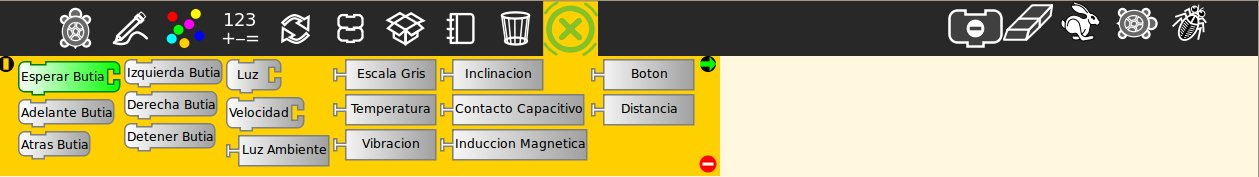
\includegraphics[scale=0.25]{graphics/paleta_butia.JPG}
		   \end{figure}
	   \end{center}
	   \begin{itemize}
	   		\item Paleta para controlar el robot
			\item<2-> Cada sensor es mostrado como un bloque
			\item<3-> Es posible ejecutar un bloque haciendo click con el rat\'on sobre el mismo cuando est\'a ubicado en el \'area de programa.
	    \end{itemize}
}

\frame {
  \frametitle{Paleta Buti\'a}
	   \begin{center}
		   \begin{figure}
		   		 Paleta Tortuga Buti\'a	
			 	 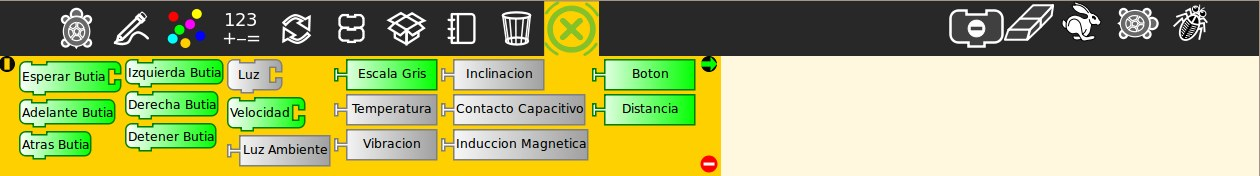
\includegraphics[scale=0.25]{graphics/paleta_butia_coloreada.JPG}
		   \end{figure}
	   \end{center}
	   \begin{itemize}
	       \item Plug \& Play: Se colorean los bloques de la paleta Buti\'a si el sensor correspondiente esta conectado
		   \item<2-> Desarrollo, depuraci\'on y ejecuci\'on sobre la misma plataforma
	    \end{itemize}
}

\frame {
  \frametitle{Programando Comportamientos}
	   \begin{center}
		   \begin{figure}
		   		 Programa para evitar obstaculos desarrollado en Tortuga	
			 	 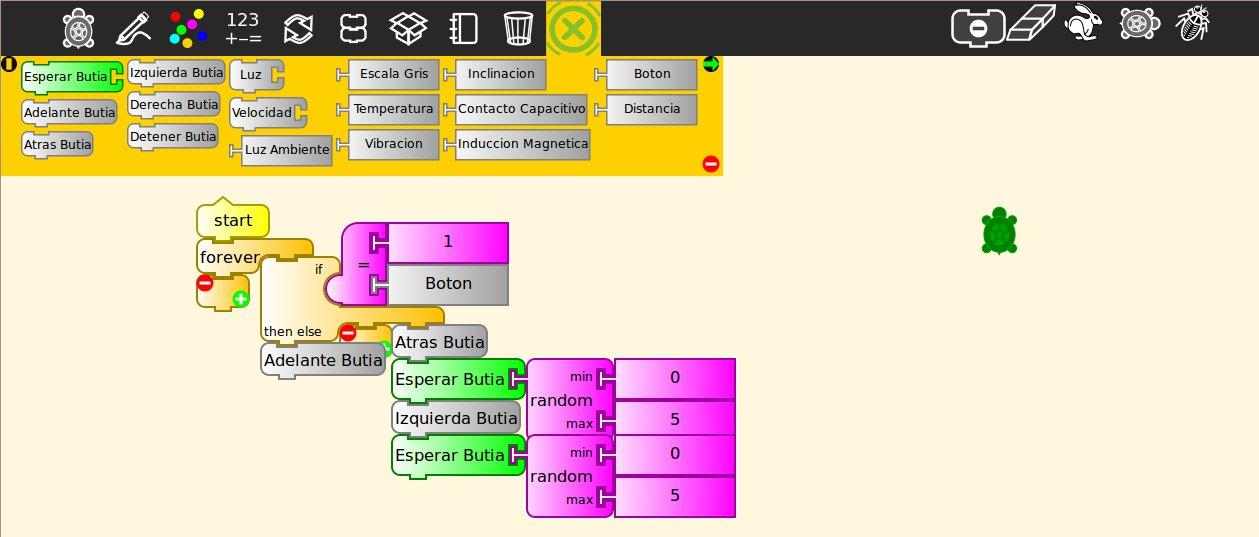
\includegraphics[scale=0.22]{graphics/tortuga_evitar_obstaculos.JPG}
		   \end{figure}
	   \end{center}
}

\frame {
  \frametitle{Programando Comportamientos}
	   \begin{center}
		   \begin{figure}
			 	 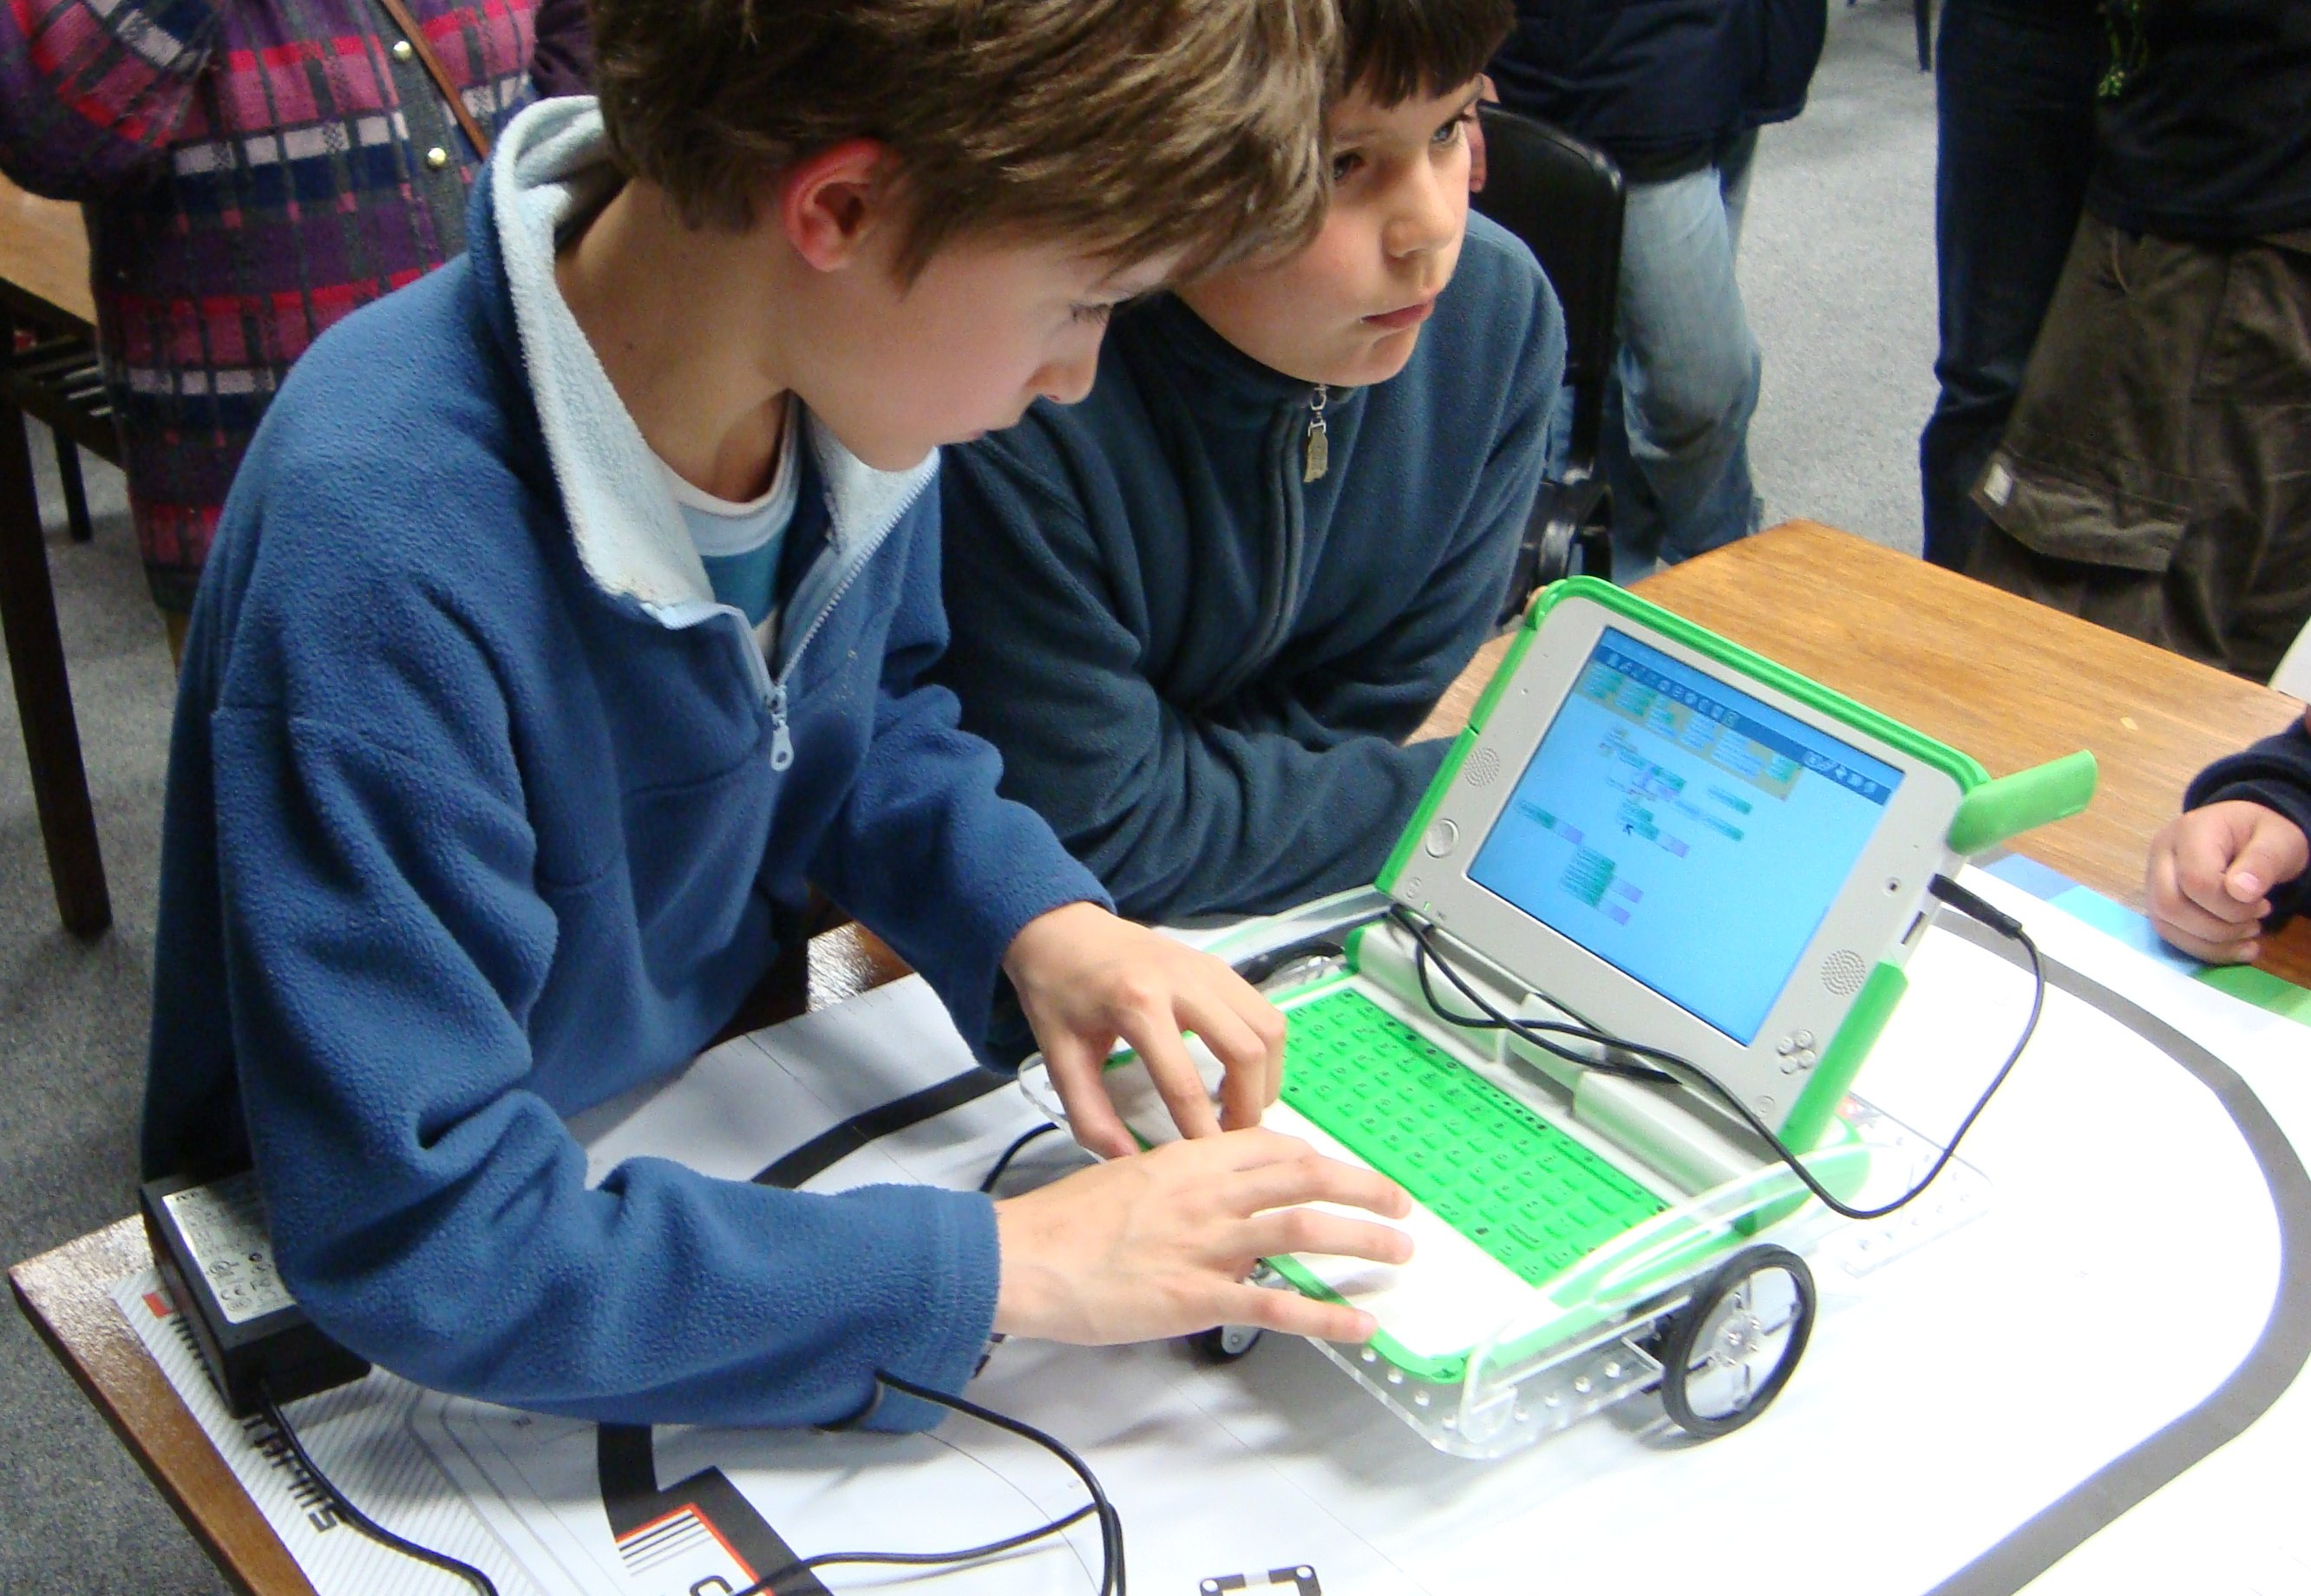
\includegraphics[scale=0.08]{graphics/pedro.JPG}
		   \end{figure}
	   \end{center}
}

\subsection{Dise\~no Mec\'anico}
%FA
\frame {
  \frametitle{Chasis constructivo}
  \begin{itemize}
 	   \item Cortes en l\'aser sobre acr\'ilico
 	   \item<2-> Superficie suficiente para llevar un netbook o XO
 	   \item<3-> Orificios para colocar los sensores o actuadores
	   \item<4-> Barandas para proteger la XO
       \item<5-> Dos ruedas de acr\'ilico las cuales est\'an sujetas a los motores
	   \item<6-> Dos ruedas locas, una de ellas amortiguada para poder sortear desniveles	
  \end{itemize}
}

\section{Implantaci\'on}
\subsection{Entrega de robots}
%AA
\frame {
  \frametitle{Entrega, visitas y apoyo en los liceos}
  \begin{itemize}
 	   \item<1-> El campeonato de sumo es un evento de rob\'otica realizado todos los a\~nos por la Facultad de Ingenier\'ia de la UdelaR 
		\begin{itemize}		
			\item<1-> En esta jornada se entregaron robots a 27 liceos seleccionados
			\item<1-> Se realiz\'o capacitaci\'on y talleres para estudiantes y profesores (81 personas aproximadamente)
		\end{itemize}
	   \item<2-> Durante los meses de octubre y noviembre se realizaron visitas a los liceos.
 	   \item<3-> Se realiz\'o capacitaci\'on y talleres para estudiantes y profesores (340 personas aproximadamente)
	   \item<4-> Cada liceo tiene un estudiante universitario como referente el cual le brinda apoyo y soporte.
  \end{itemize}
}

\section{Conclusiones y trabajo a futuro}
% AA
\subsection{...Buti\'a 2.0}
\frame {
\frametitle{Trabajo futuro}
 \begin{itemize}
  	\item Disminuir costos.
   	\item<2-> Portar a otros lenguajes gr\'aficos como Scratch
 	\item<3-> Ser m\'as eficientes con el uso de los pines para identificaci\'on
 	\item<4-> Culminar la implementaci\'on de plug \& play y shield para placa USB4all (microcontrolador PIC)
	\item<5-> Mejorar aspectos constructivos
	\item<6-> Continuar mejorando la estabilidad
	\item<7-> Buti\'a con elementos de desecho
	\item<8-> Incluir un brazo rob\'otico en el kit
	\end{itemize}
}

\subsection{finalmente...}
%FA
\frame {
\frametitle{Conclusiones}
 \begin{itemize}
   \item Se realiz\'o un prototipo de robot, constructivo, totalmente integrado a la computadora utilizada por OLPC y su sistema SUGAR
   \item<2-> Se implat\'o en 27 liceos del pa\'is
   \item<3-> Pudo validarse que incluso ni\~nos pueden programar comportamiento de robots f\'acilmente y sin conocimientos previos
   \item<4-> El proyecto tuvo un gran impacto en todo el pa\'is y permiti\'o obtener informaci\'on a partir de su puesta en pr\'actica
  \end{itemize}
}

\section{Presentaci\'on del curso}
\subsection{MTButi\'a}
\frame {
\frametitle{Curso}
 \begin{itemize}
       \begin{figure}
			 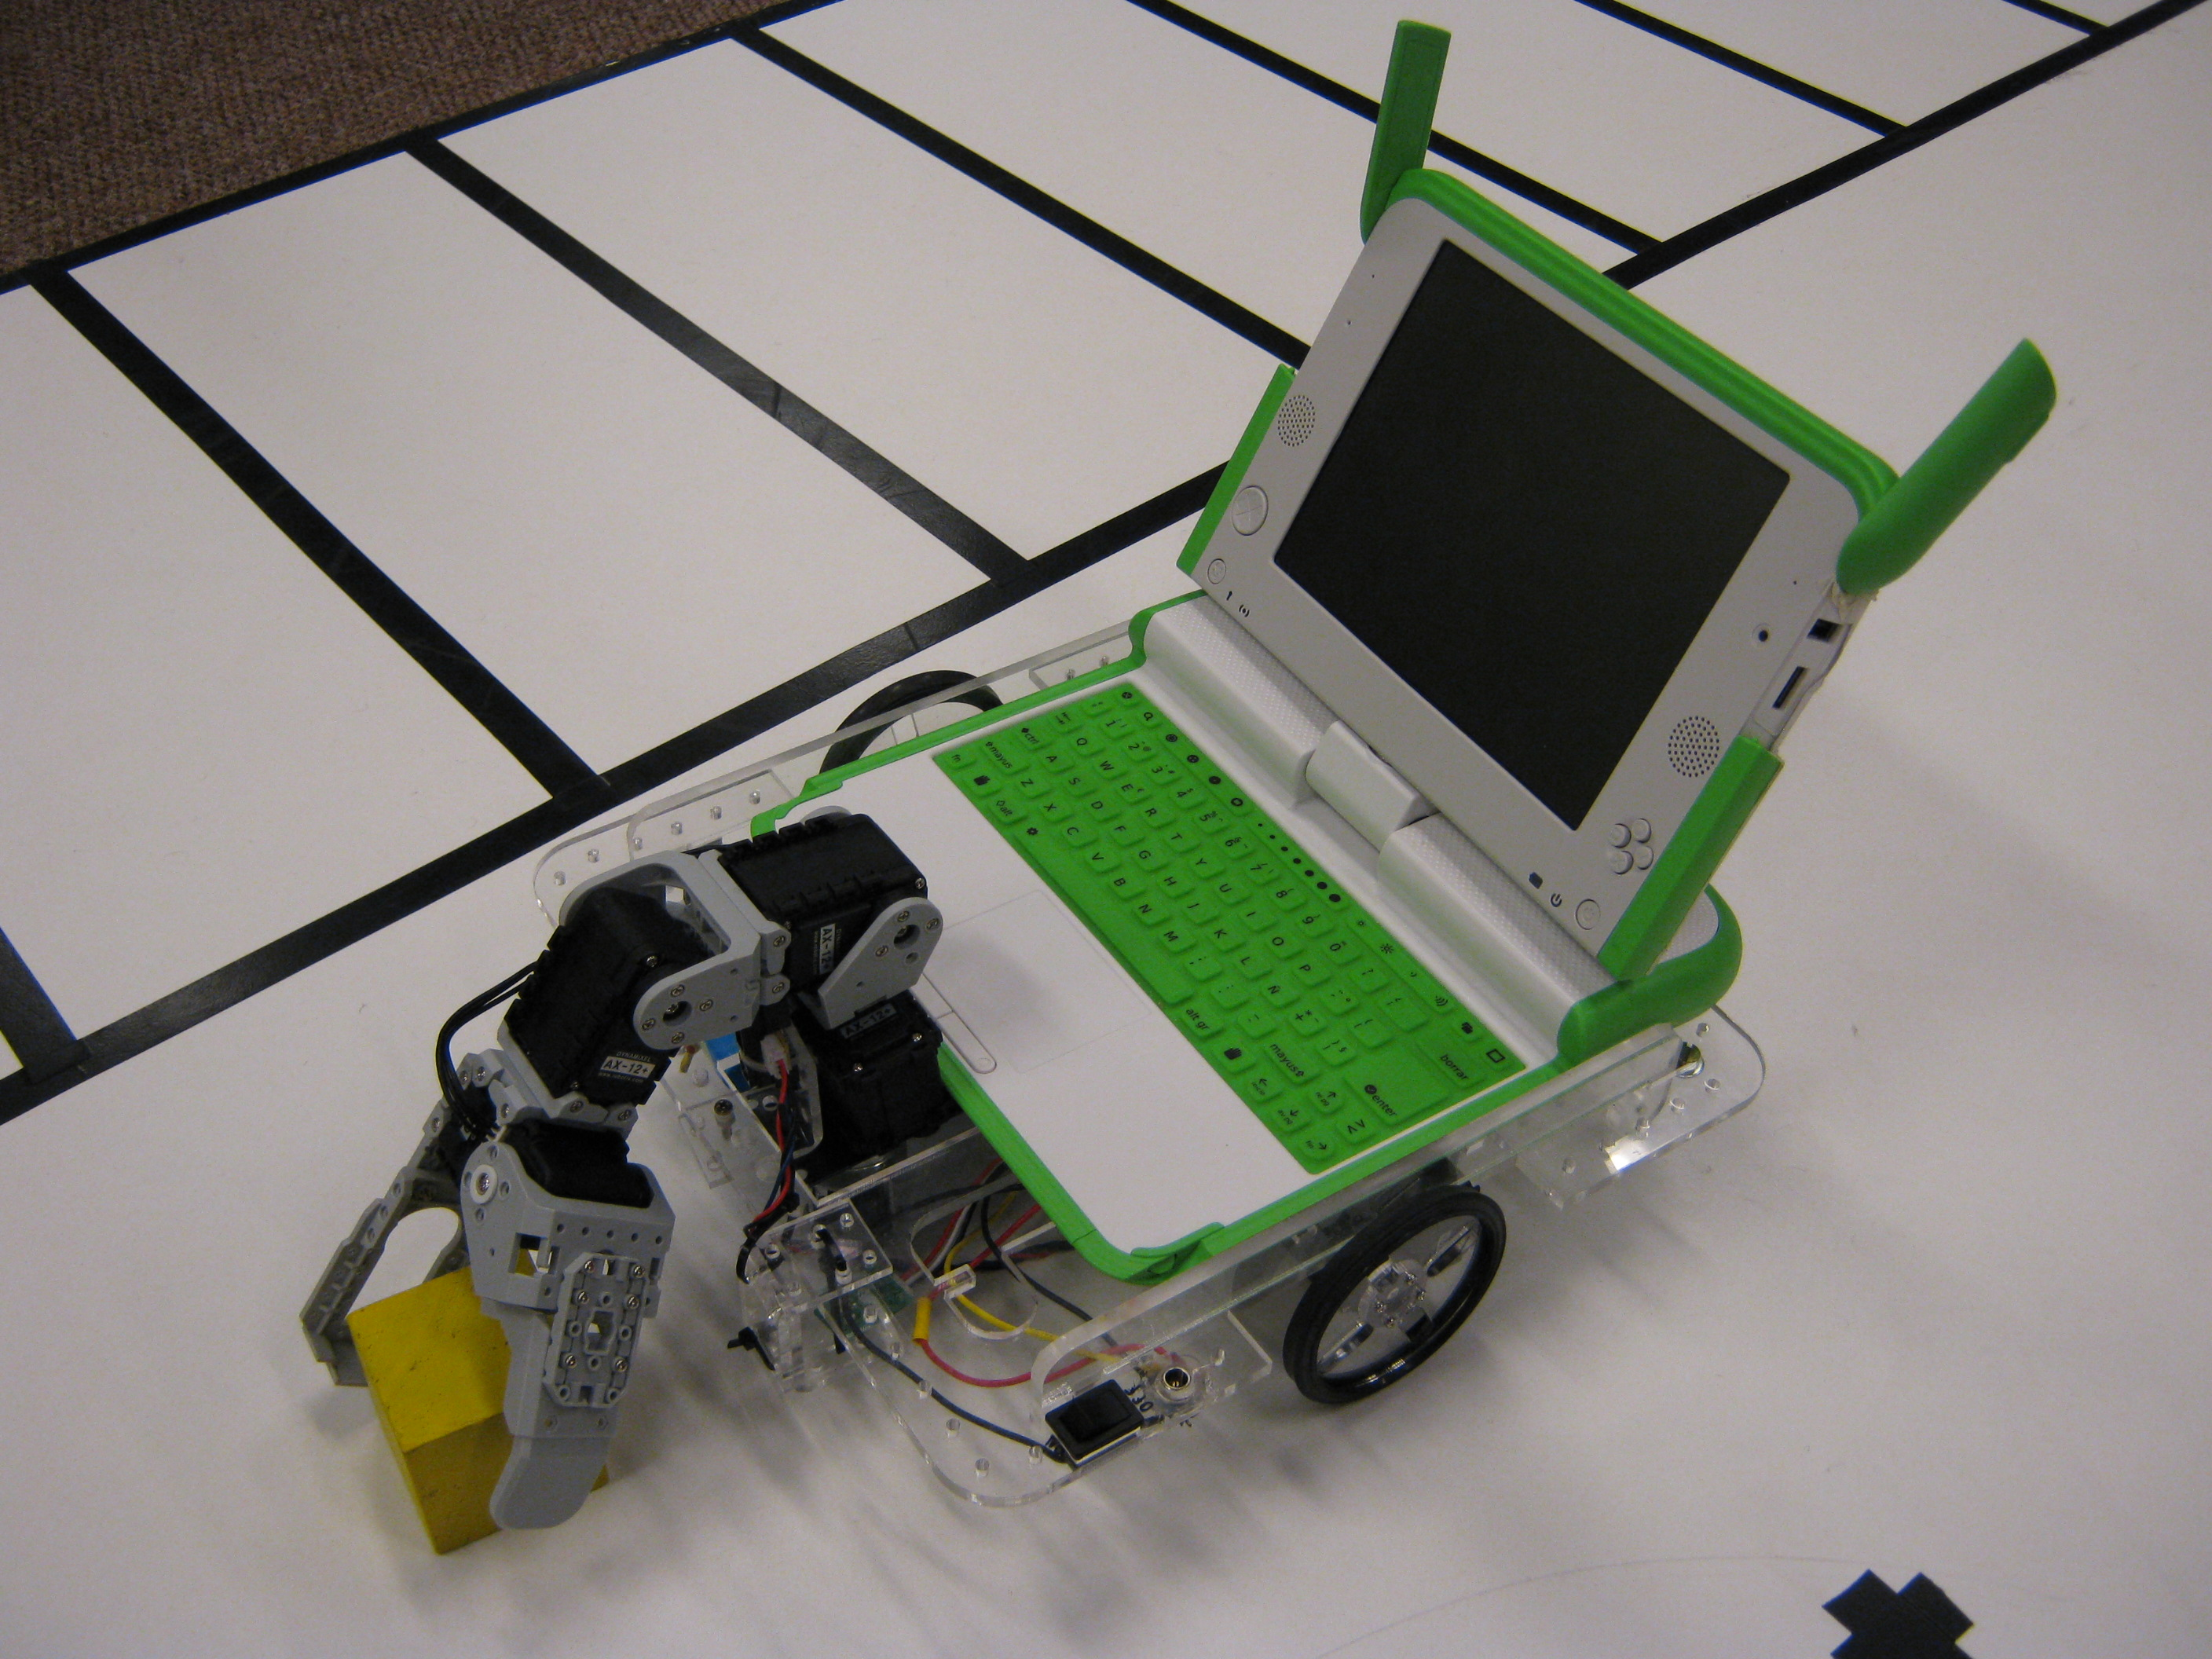
\includegraphics[scale=0.05]{graphics/butia_pinza.JPG}
	   \end{figure}
  	\item Curso MTButi\'a.
 \end{itemize}
}

\subsection{MTButi\'a}
\frame {
\frametitle{Objetivo}
 \begin{itemize}
  	\item Controlar y extender las funcionalidades del robot Buti\'a.
   	\item<2-> Trabajar junto a docentes y estudiantes de secundaria de todo el pa\'is en la ense\~nanza de la inform\'atica utilizando robots m\'oviles.
 	\item<3-> Comprender los principios de funcionamiento y construcci\'on de robots m\'oviles.
 	\item<4-> Conocer los principales lenguajes de programaci\'on incluidos en las computadoras XO del plan Ceibal.	
	\end{itemize}
}

\frame {
\frametitle{Temario}
 \begin{itemize}
  	\item Introducci\'on e historia de la rob\'otica.
   	\item<2-> Construcci\'on de robots.
 	\item<3-> Presentaci\'on de la XO.
	\item<4-> Lenguajes de programaci\'on.
    \item<5-> Single Boards Computers.
    \item<6-> El robot Buti\'a.
	\end{itemize}
}

\frame {
\frametitle{Forma de trabajo}
 \begin{itemize}
  	\item El curso es principalmente trabajo de laboratorio y de campo, con algunas presentaciones te\'oricas.
   	\item<2-> Se trabajar\'a sobre el robot buti\'a, extendiendo alguna caracter\'istica.
 	\item<3-> Cada estudiante ser\'a referente de un liceo:
    \begin{itemize}		
			\item<3-> Capacitaci\'on.
			\item<3-> Apoyo durante el proyecto.
            \item<3-> Coordinar la participaci\'on al evento Sumo.uy 2011 y apoyo durante el mismo.
		\end{itemize}
\end{itemize}
}

\frame {
\frametitle{Dedicaci\'on}
 \begin{itemize}
  	\item 18 semanas aproximadamente.
   	\item<2-> 6 cr\'editos.
 	\item<3-> 4 horas semanales. 	
	\end{itemize}
}

\frame {
\frametitle{Horarios}
 \begin{itemize}
  	\item Te\'orico:
    \begin{itemize}		
			\item Lunes de 18:00 a 19:30hs. sal\'on 301
            \item Mi\'ercoles de 18:00 a 19:30hs. sal\'on 301.			 
		\end{itemize}
    \item<2-> Laboratorio:
    \begin{itemize}		
			\item<2-> Lunes de 18:00 a 20:00hs. laboratorio de rob\'otica.
			\item<2-> Mi\'ercoles de 18:00 a 20:00hs. laboratorio de rob\'otica.
		\end{itemize}
\end{itemize}
}

\frame {
\frametitle{Aprobaci\'on}
 \begin{itemize}
  	\item Asistencia obligatoria al te\'orico y al laboratorio.
  	\item<2-> Realizaci\'on de ejercicios de laboratorio.
	\item<3-> Extensi\'on de las funcionalidades del Buti\'a.
    \begin{itemize}		
			\item<3-> Implementaci\'on.
			\item<3-> Reporte t\'ecnico.
            \item<3-> Prueba del laboratorio en el entorno definido.
            \item<3-> Presentaci\'on.
	\end{itemize}
\end{itemize}
}

\frame {
\frametitle{Evaluaci\'on}
 \begin{itemize}
  	\item Puntajes de evaluaci\'on:   	
    \begin{itemize}		
			\item Laboratorio 60 \%.
			\item Presentaci\'on: 40 \%.            
	\end{itemize}
    \item<2-> La aprobaci\'on corresponde al 60 \% de la evaluaci\'on total.
\end{itemize}
}

\frame {
\frametitle{Cupo}
\begin{itemize}
 	\item 30 personas.
    \item<2-> El criterio para ordenar los estudiantes se basar\'a en:
   \begin{itemize}		
			\item<2-> asistencia a las clases introductorias.
			\item<2-> avance en la carrera y sorteo.
	\end{itemize}
\end{itemize}
}

\frame {
  \frametitle{Gracias}
{Preguntas?}
   \begin{center}
	   \begin{figure}
			 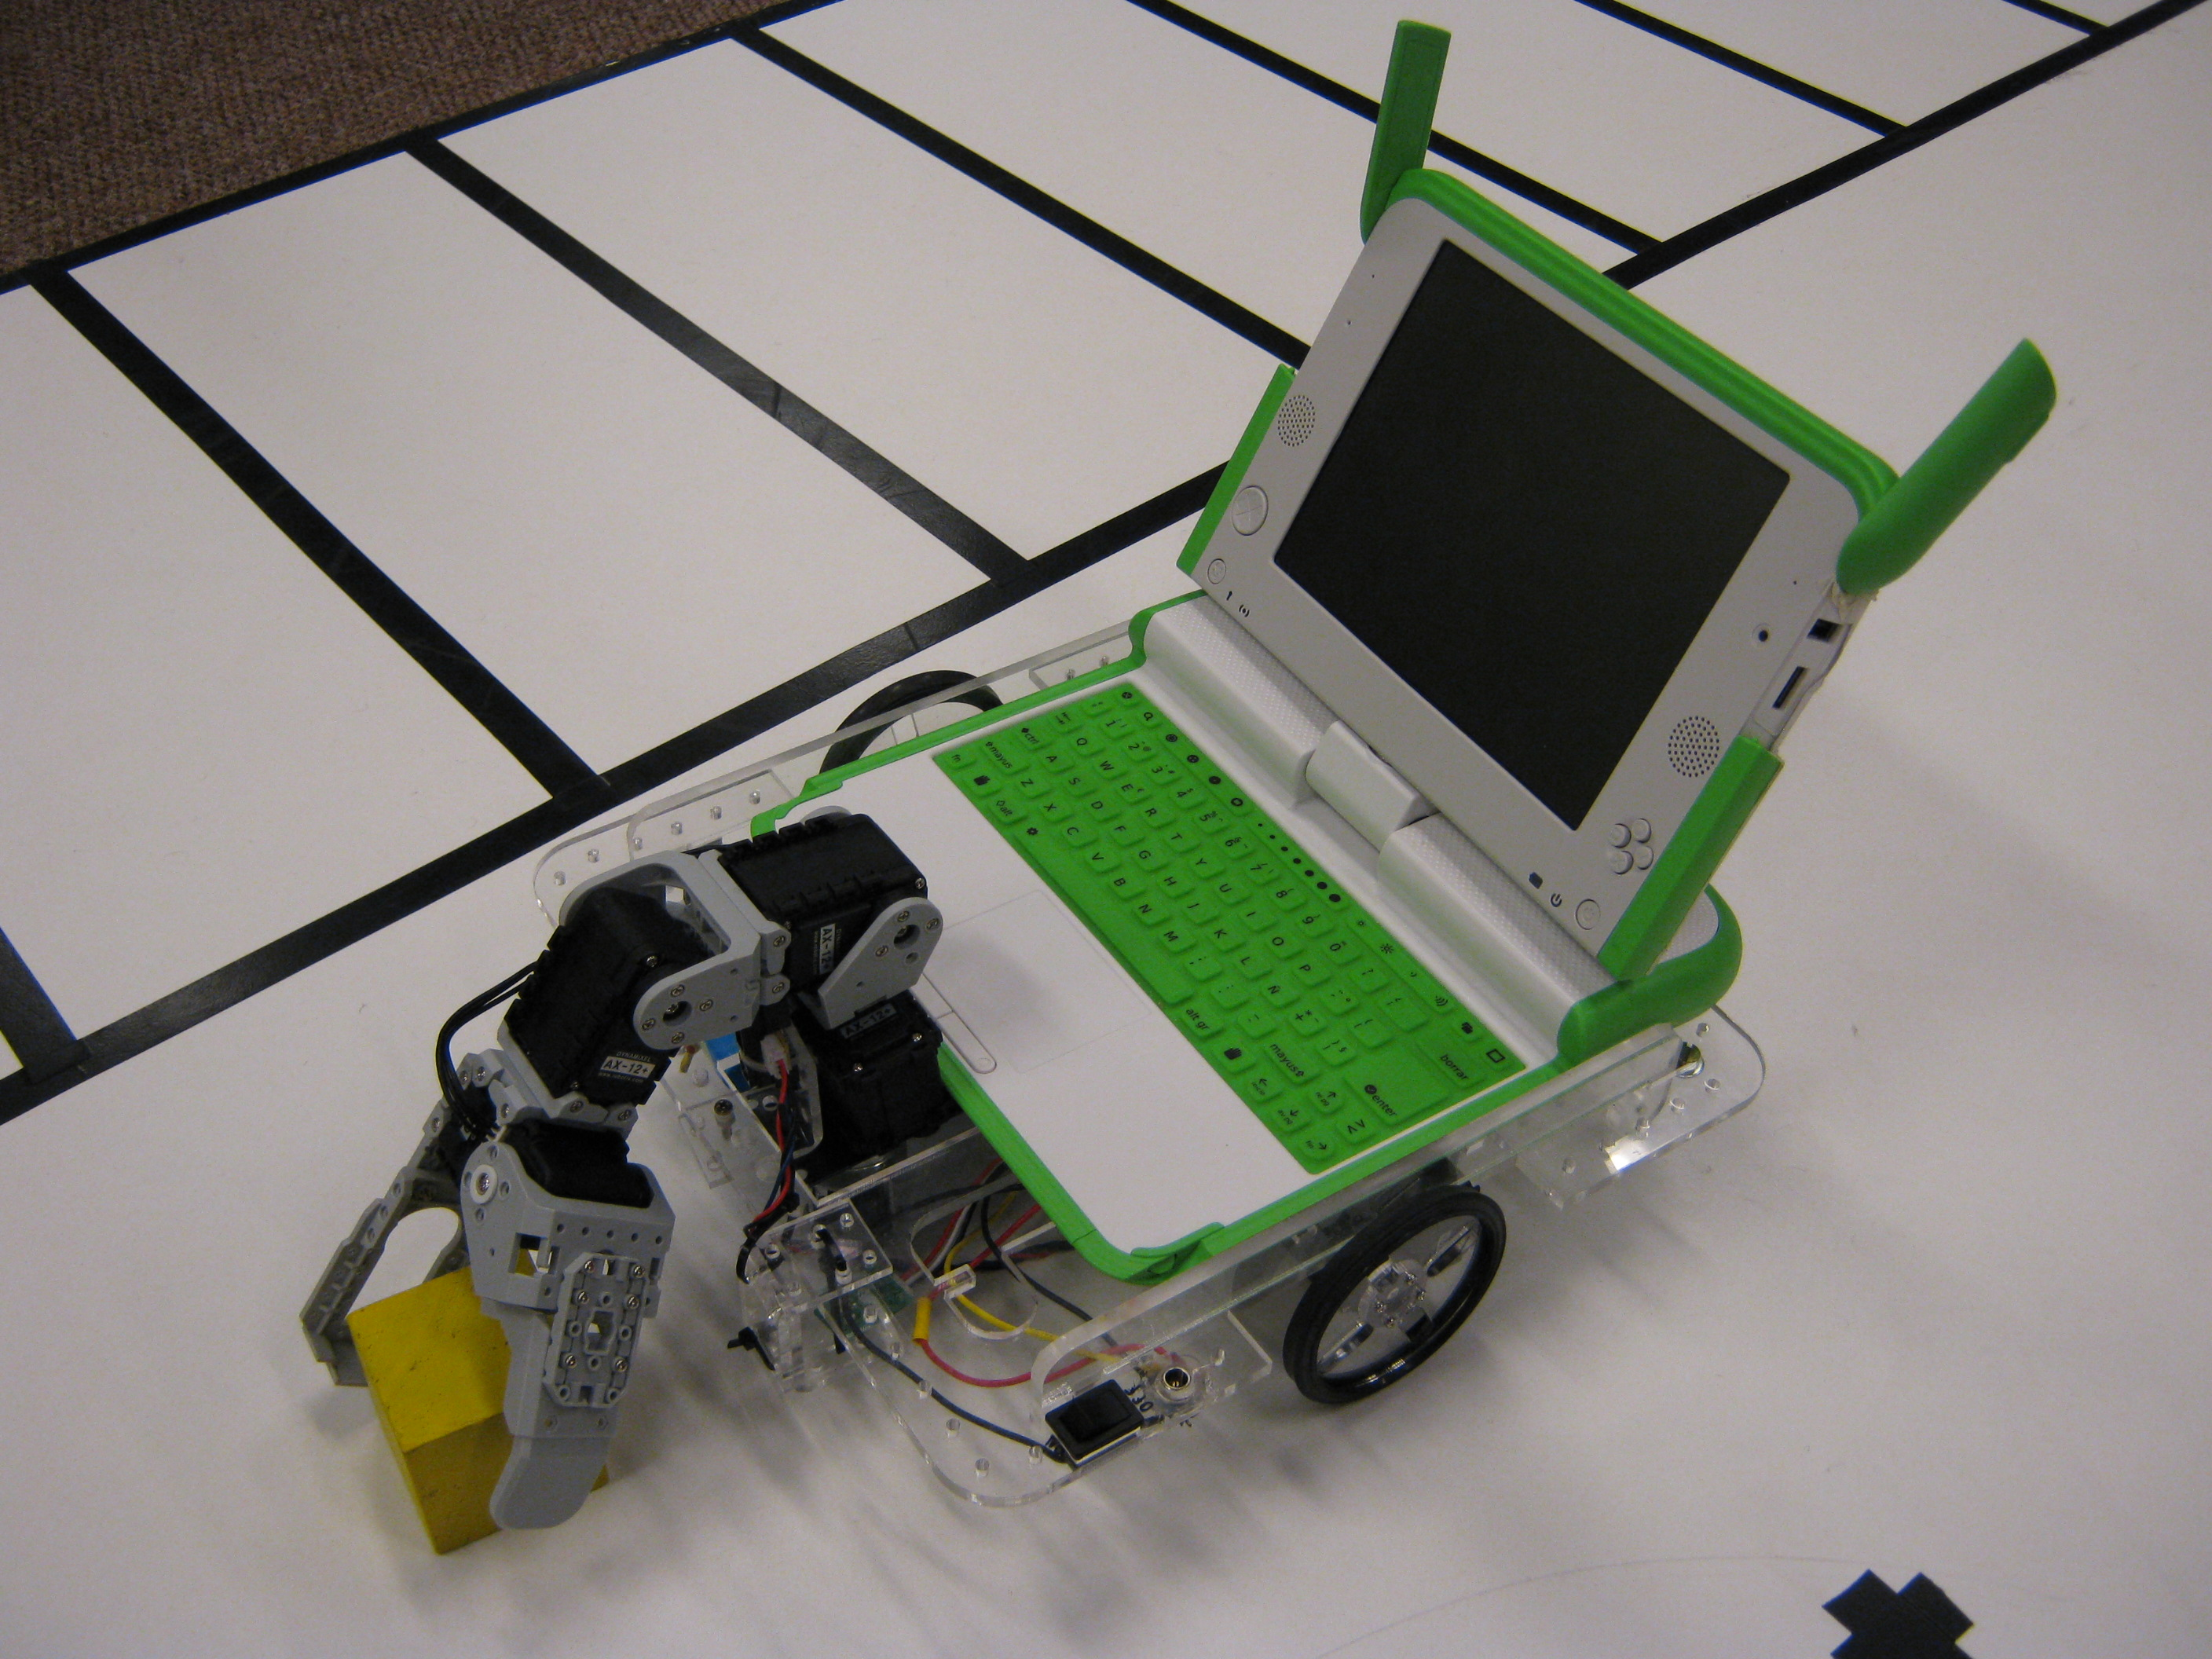
\includegraphics[scale=0.05]{graphics/butia_pinza.JPG}
	   \end{figure}
    \item mail: butia@fing.edu.uy
    \item news: fing.cursos.mtbutia (news.fing.edu.uy).
    \item web: http://www.fing.edu.uy/inco/proyectos/butia/ (secci\'on curso)
   \end{center}  
}
\frame{\titlepage}

%\setbeamertemplate{background canvas}{\includegraphics[width=\paperwidth]{{graphics/bsod2.jpg}}}
%\begin{frame}[plain]
%\begin{centering}%
%\par%
%\end{centering}%
%\end{frame}

\end{document}

